% !TeX root = main.tex
\documentclass{beamer}
\usetheme{Copenhagen}
%\usecolortheme{whale}
\setbeamertemplate{itemize item}[triangle]
\setbeamertemplate{itemize subitem}[square]
\useoutertheme{infolines}
\usepackage{xcolor}
\usepackage{tikz}
\usepackage{comment}
\usepackage{appendixnumberbeamer}
\usetikzlibrary{arrows, arrows.meta,calc,automata,fit,shapes,positioning}
\tikzset{AUT style/.style={>=angle 60,initial text= ,every edge/.append,every state/.style={minimum size=20,inner sep=2}}}

\definecolor{RealGreen}{HTML}{33bb33}
\definecolor{DarkGreen}{HTML}{338833}

\newcommand{\messages}{\mathcal{M}}
\newcommand{\br}{\mathbf{br}}
\newcommand{\rec}{\mathbf{rec}}
\newcommand{\reg}{\hspace{-0.5mm}\square}
%
%\setbeamertemplate{section in toc}[square]
\setbeamercolor{section number projected}{bg=black,fg=white}

\begin{document}
	
	\title[]{Parameterized verification of Broadcast networks of Register automata}
	\date[]{January 16th, 2024}
	\author[Nicolas Waldburger]{Nicolas Waldburger\\ joint work with Lucie Guillou and Corto Mascle}
	\institute[]{ANR PaVeDyS}
	\setbeamertemplate{navigation symbols}{}
	\addtobeamertemplate{title page}{}{\begin{center}{To be published at FoSSaCS'24}\end{center}}
%	
\begin{frame}
	\titlepage
\end{frame}	

\begin{frame}
	\tableofcontents
\end{frame}

\section{Broadcast networks}

\subsection{Basic model}

\begin{frame}
	\tableofcontents[currentsection]
\end{frame}


\begin{frame}{Broadcast networks}
	\centering
	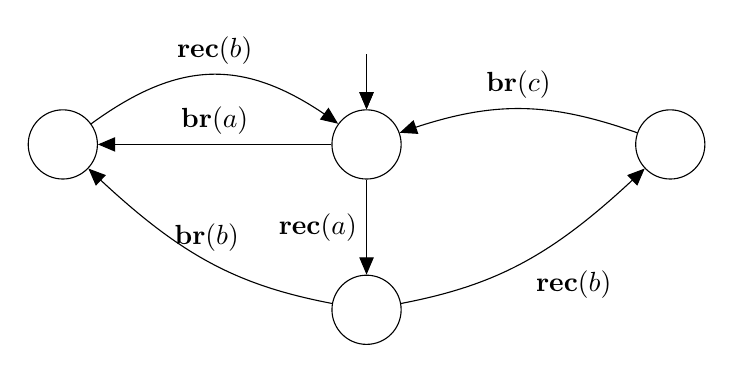
\begin{tikzpicture}[xscale=0.5,node distance=2.1cm,auto,>= triangle
	45]
	\tikzstyle{initial}= [initial by arrow,initial text=,initial
	distance=.7cm, initial above]
	%	\tikzstyle{accepting}= [accepting by arrow,accepting text=,accepting
	%	distance=.7cm,accepting where =right]
	
	\node[state,initial, minimum width=0.1pt] (0) at (0,0) {};
	\node[state] [left of=0, xshift=-50] (x) {};
	\node[state] [below of=0] (y) {};
	\node[state] [right of=0, xshift=50] (z) {};
	
\path[->, bend left=20] (x) edge node[above] {$\mathbf{rec}(b)$} (0);
	
	
	\path[->, bend left=10] 	
	(y) edge node[above] {$\mathbf{br}(b)$} (x)
	;
	
	\path[->] 	
	(0) edge node[left] {$\mathbf{rec}(a)$} (y)
	;
	
	\path[->](0) edge node[above] {$\mathbf{br}(a)$} (x);
	
	\path[->, bend right=10] 	
	(y) edge node[below right] {$\mathbf{rec}(b)$} (z)
	(z) edge node[above] {$\mathbf{br}(c)$} (0)
	;
\end{tikzpicture}
\end{frame}


\begin{frame}{Broadcast networks}
	\centering
	\hspace{-4cm}
\resizebox{5cm}{2.2cm}{
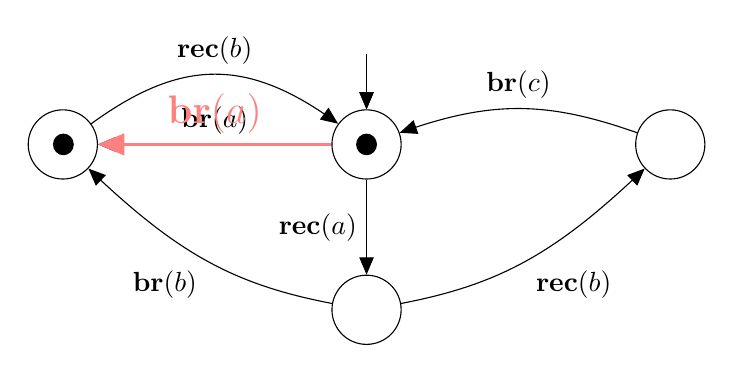
\begin{tikzpicture}[xscale=0.5,node distance=2.1cm,auto,>= triangle
	45]
	\tikzstyle{initial}= [initial by arrow,initial text=,initial
	distance=.7cm, initial above]
	%	\tikzstyle{accepting}= [accepting by arrow,accepting text=,accepting
	%	distance=.7cm,accepting where =right]
	
	\node[state,initial, minimum width=0.1pt] (0) at (0,0) {};
	\node[state] [left of=0, xshift=-50] (x) {};
	\node[state] [below of=0] (y) {};
	\node[state] [right of=0, xshift=50] (z) {};
	
	\onslide<1>{\draw[fill=black] (0,0) ellipse (0.25 and 0.13);}
	\onslide<2->{\draw[fill=black] (-7.7,0) ellipse (0.25 and 0.13);}
	
	\path[->, bend left=10] 	
	(y) edge node[below left] {$\mathbf{br}(b)$} (x)
	;
	
	\path[->, bend left=20] (x) edge node[above] {$\mathbf{rec}(b)$} (0);
	
	
	\path[->] 	
	(0) edge node[left] {$\mathbf{rec}(a)$} (y)
	;
	
	\onslide<1,3->{\path[->](0) edge node[above] {$\mathbf{br}(a)$} (x);}
	\onslide<2>{\path[->, very thick, red!50] (0) edge node[above] {\Large $\mathbf{br}(a)$} (x);}
	
	\path[->, bend right=10] 	
	(y) edge node[below right] {$\mathbf{rec}(b)$} (z)
	(z) edge node[above] {$\mathbf{br}(c)$} (0)
	;
\end{tikzpicture}
}

\hspace{4cm}
\resizebox{5cm}{2.2cm}{
	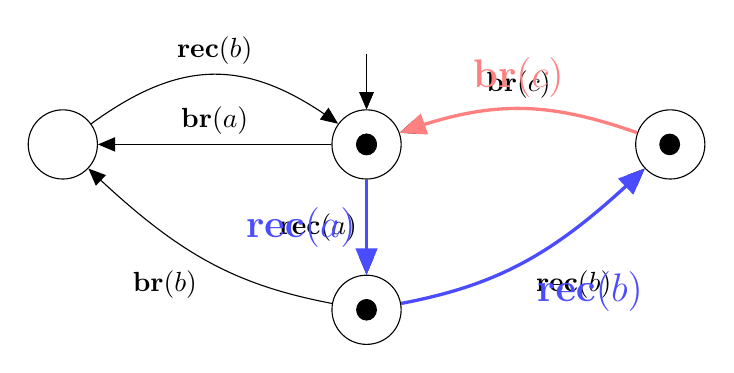
\begin{tikzpicture}[xscale=0.5,node distance=2.1cm,auto,>= triangle
		45]
		\tikzstyle{initial}= [initial by arrow,initial text=,initial
		distance=.7cm, initial above]
		%	\tikzstyle{accepting}= [accepting by arrow,accepting text=,accepting
		%	distance=.7cm,accepting where =right]
		
		\node[state,initial, minimum width=0.1pt] (0) at (0,0) {};
		\node[state] [left of=0, xshift=-50] (x) {};
		\node[state] [below of=0] (y) {};
		\node[state] [right of=0, xshift=50] (z) {};
		
		
		\onslide<2>{\draw[fill=black] (0,-2.1) ellipse (0.25 and 0.13);}
		\onslide<3>{\draw[fill=black] (7.7,0) ellipse (0.25 and 0.13);}
		\onslide<1>{\draw[fill=black] (0,0) ellipse (0.25 and 0.13);}
		\onslide<4>{\draw[fill=black] (0,0) ellipse (0.25 and 0.13);}
		
\path[->, bend left=20] (x) edge node[above] {$\mathbf{rec}(b)$} (0);
		
			\onslide<1-4>{\path[->,bend left=10](y) edge node[below left] {$\mathbf{br}(b)$} (x);}
		
		\onslide<1-2,4>{\path[->,bend right=10](y) edge node[below right] {$\mathbf{rec}(b)$} (z);}
		\onslide<3>{\path[->, very thick,bend right=10, blue!70] (y) edge node[below right] {\Large $\mathbf{rec}(b)$} (z);}
		
		\onslide<1-3>{\path[->,bend right=10](z) edge node[above] {$\mathbf{br}(c)$} (0);}
		\onslide<4>{\path[->, very thick,bend right=10, red!50] (z) edge node[above] {\Large $\mathbf{br}(c)$} (0);}
		
		\path[->] 	
		(0) edge node[above] {$\mathbf{br}(a)$} (x)
		;
		
		\onslide<1,3->{\path[->](0) edge node[left] {$\mathbf{rec}(a)$} (y);}
		\onslide<2>{\path[->, very thick, blue!70] (0) edge node[left] {\Large $\mathbf{rec}(a)$} (y);}
		;
	\end{tikzpicture}
}

\hspace{-4cm}
\resizebox{5cm}{2.2cm}{
	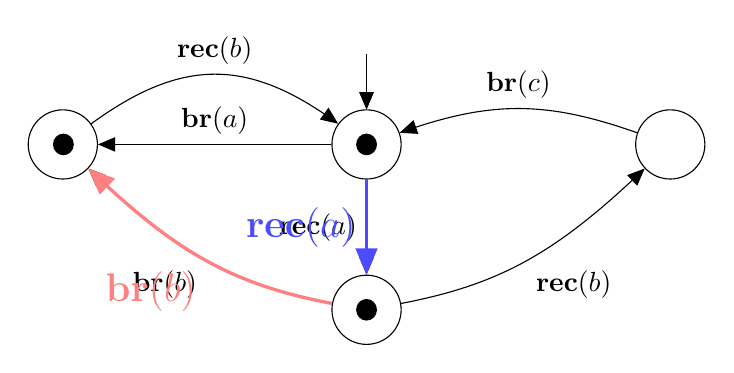
\begin{tikzpicture}[xscale=0.5,node distance=2.1cm,auto,>= triangle
		45]
		\tikzstyle{initial}= [initial by arrow,initial text=,initial
		distance=.7cm, initial above]
		%	\tikzstyle{accepting}= [accepting by arrow,accepting text=,accepting
		%	distance=.7cm,accepting where =right]
		
		\node[state,initial, minimum width=0.1pt] (0) at (0,0) {};
		\node[state] [left of=0, xshift=-50] (x) {};
		\node[state] [below of=0] (y) {};
		\node[state] [right of=0, xshift=50] (z) {};
		
		\onslide<1>{\draw[fill=black] (0,0) ellipse (0.25 and 0.13);}
		\onslide<2>{\draw[fill=black] (0,-2.1) ellipse (0.25 and 0.13);}
		\onslide<3->{\draw[fill=black] (-7.7,0) ellipse (0.25 and 0.13);}

		
		\path[->] 	
		(0) edge node[above] {$\mathbf{br}(a)$} (x)
		;
\path[->, bend left=20] (x) edge node[above] {$\mathbf{rec}(b)$} (0);
		
		
		\onslide<1,3->{\path[->](0) edge node[left] {$\mathbf{rec}(a)$} (y);}
		\onslide<2>{\path[->, very thick, blue!70] (0) edge node[left] {\Large $\mathbf{rec}(a)$} (y);}
		
		\onslide<1-2,4>{\path[->,bend left=10](y) edge node[below left] {$\mathbf{br}(b)$} (x);}
		\onslide<3>{\path[->, very thick,bend left=10, red!50] (y) edge node[below left] {\Large $\mathbf{br}(b)$} (x);}
		
		
		\path[->, bend right=10] 	
		(y) edge node[below right] {$\mathbf{rec}(b)$} (z)
		(z) edge node[above] {$\mathbf{br}(c)$} (0)
		;
	\end{tikzpicture}
}
\end{frame}

\begin{frame}{Broadcast Networks}
	\begin{block}{Definition$^1$}
		(Reconfigurable) Broadcast Network = $(Q, M, \Delta, q_0)$ with $\Delta \subseteq Q\times \{\mathbf{br}(m), \mathbf{rec}(m) \mid m \in M\} \times Q$.
	\end{block}
	
	\pause
	
	\begin{itemize}
		\item Arbitrarily many agents at the start
		
		\item One step = an agent broadcasts a message $m$,\\ some (arbitrary subset of) other agents receive it.
	\end{itemize}
	
	\pause 
	
	\begin{block}{Problems}
%		\vspace{0.3cm}
		{\sc{Cover}}: Is there a run in which \textbf{an} agent reaches \color{blue!60}$q_f$\color{black}?
%		\vspace{0.3cm}
		
		{\sc{Target}}: Is there a run in which \textbf{all agents} reach \color{blue!60}$q_f~$\color{black} \textbf{simultaneously}?
	\end{block}
	
	Both problems are decidable in PTIME\footnote{Delzanno, Sangnier, Zavattaro, CONCUR'10}\footnote{Delzanno, Sangnier, Traverso, Zavattaro, FSTTCS'12}.
\end{frame}

\subsection{With registers}

\begin{frame}
	\tableofcontents[currentsubsection]
\end{frame}

\begin{frame}{Registers}
	
	Each agent now has local registers $\reg_1, \ldots, \reg_r$, containing values in $\mathbb{N}$.\vspace{0.3cm}\pause
	
	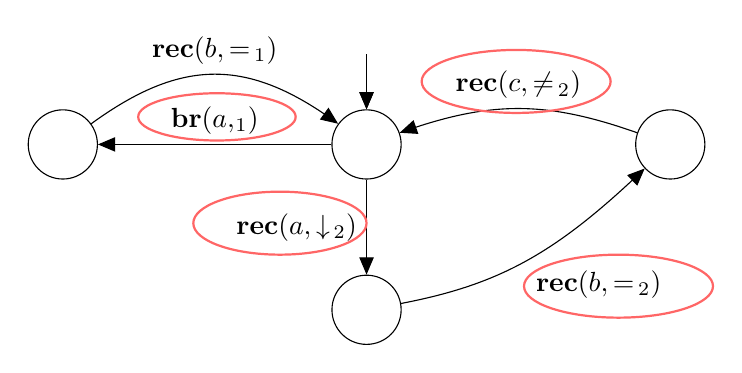
\begin{tikzpicture}[xscale=0.5,node distance=2.1cm,auto,>= triangle
	45]
	\tikzstyle{initial}= [initial by arrow,initial text=,initial
	distance=.7cm, initial above]
	%	\tikzstyle{accepting}= [accepting by arrow,accepting text=,accepting
	%	distance=.7cm,accepting where =right]
	
	\node[state,initial, minimum width=0.1pt] (0) at (0,0) {};
	\node[state] [left of=0, xshift=-50] (x) {};
	\node[state] [below of=0] (y) {};
	\node[state] [right of=0, xshift=50] (z) {};
	
	\path[->, bend left=20] (x) edge node[above] {$\mathbf{rec}(b, =\reg_1)$} (0);
	
%	\path[->, bend left=10] 	
%	(y) edge node[above] {$\mathbf{br}(b)$} (x)
%	;
	
	\path[->] 	
	(0) edge node[left] {$\mathbf{rec}(a, \downarrow \reg_2)$} (y)
	;
	
	\path[->](0) edge node[above] {$\mathbf{br}(a, \reg_1)$} (x);
	
	\path[->, bend right=10] 	
	(y) edge node[below right] {$\mathbf{rec}(b, = \reg_2)$} (z)
	(z) edge node[above] {$\mathbf{rec}(c, \neq \reg_2)$} (0)
	;
	
	\onslide<2>
	{
	\draw[color=red!60,thick] (-3.8,0.35) ellipse (2 and 0.3);
	}
	\onslide<3>
	{
		\draw[color=red!60,thick] (-2.2,-1) ellipse (2.2 and 0.4);
	}
	
	\onslide<4>
	{
		\draw[color=red!60,thick] (6.4,-1.8) ellipse (2.4 and 0.4);
	}
	
	\onslide<5>
	{
		\draw[color=red!60,thick] (3.8,0.8) ellipse (2.4 and 0.4);
	}
\end{tikzpicture}
\end{frame}

\begin{frame}{Broadcast Networks of Register Automata (BNRA)\footnote{Delzanno, Sangnier, Traverso, RP'13}}
	Each agent now has local \emph{registers} $\reg_1, \ldots, \reg_r$, containing values in $\mathbb{N}$.
	\pause
	\textbf{Initially, all registers of all agents contain distinct values.}
	
	\pause
	\vspace{0.2cm}
	Messages also contain values: $(m, v) \in M\times \mathbb{N}$.
	An agent can:
	\begin{itemize}
		\item Broadcast a message with a register value $\mathbf{br}(m, r_i)$\vspace{0.3cm}\pause
		
%		\item Test equality between its registers $\mathbf{loc}(r_i, r_j, =), \mathbf{loc}(r_i, r_j, \neq)$\pause
		
		\item Receive messages $\mathbf{rec}(m, r_i, op)$, with $op$ either
		\begin{itemize}
			\item store the value $\downarrow$,
			
			\item test it for equality $=, \neq$
			
			\item or do nothing $*$.
		\end{itemize}   
	\end{itemize}
\end{frame}

\begin{frame}{Things we can do}
	
	We can check that a sequence of messages all come from the same agent.

	\begin{center}
	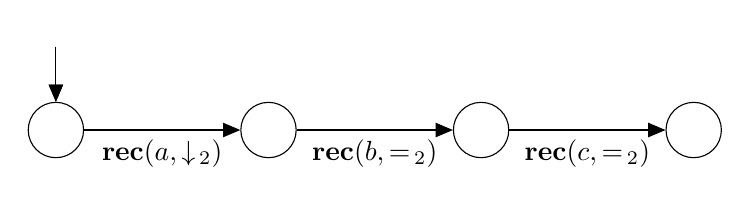
\begin{tikzpicture}[xscale=0.5,node distance=2.7cm,auto, AUT style,>= triangle
	45]
	\tikzstyle{initial}= [initial by arrow,initial text=,initial
	distance=.7cm, initial above]
	%	\tikzstyle{accepting}= [accepting by arrow,accepting text=,accepting
	%	distance=.7cm,accepting where =right]
	
	\node[state, initial, minimum width=0.1pt] (0) at (0,0) {};
	\node[state] [right of=0] (y) {};
	\node[state] [right of=y] (z) {};
	\node [state, right of = z] (s) {};
	
	
	%	\path[->, bend left=10] 	
	%	(y) edge node[above] {$\mathbf{br}(b)$} (x)
	%	;
	
	% \path[->, loop above] (z) edge node[above] {$\rec(a, =\reg_2)$} (z);
	
	\path[->] 	
	(0) edge node[below] {$\mathbf{rec}(a, \downarrow \reg_2)$} (y)
	(y) edge node[below] {$\mathbf{rec}(b, = \reg_2)$} (z)
	(z) edge node[below] {$\mathbf{rec}(c, = \reg_2)$} (s)
	;
	
\end{tikzpicture}
	\end{center}
\end{frame}

\begin{frame}{Things we can do}
	We can check that a sequence of messages we sent was received.
	
	\centering
		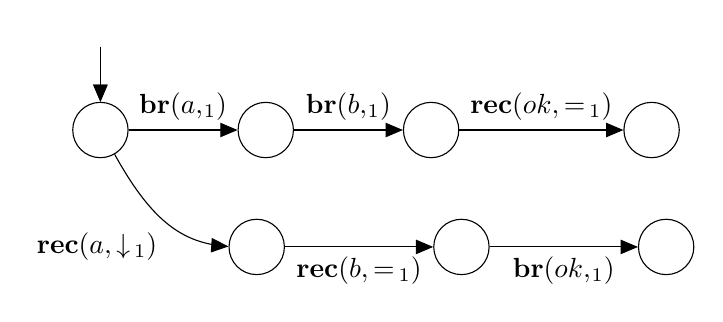
\begin{tikzpicture}[xscale=0.5,node distance=2.1cm,auto, AUT style,>= triangle
	45]
	\tikzstyle{initial}= [initial by arrow,initial text=,initial
	distance=.7cm, initial above]
	%	\tikzstyle{accepting}= [accepting by arrow,accepting text=,accepting
	%	distance=.7cm,accepting where =right]
	
	\node[state, initial, minimum width=0.1pt] (0) at (0,0) {};
	\node[state] [right of=0] (x) {};
	\node[state] [right of=x] (y) {};
	\node[state] [right of=y, xshift=0.7cm] (z) {};
	
	\node[state] [below right of=0, xshift=0.5cm] (x') {};
	\node[state] [right of=x', xshift=0.5cm] (y') {};
	\node[state] [right of=y',xshift=0.5cm] (z') {};
	
	
	%	\path[->, bend left=10] 	
	%	(y) edge node[above] {$\mathbf{br}(b)$} (x)
	%	;
	
	
	\path[->] 	
	(0) edge node[above] {$\mathbf{br}(a, \reg_1)$} (x)
	(x) edge node[above] {$\mathbf{br}(b, \reg_1)$} (y)
	(y) edge node[above] {$\mathbf{rec}(ok, = \reg_1)$} (z)
	(x') edge node[below] {$\mathbf{rec}(b, = \reg_1)$} (y')
	(y') edge node[below] {$\mathbf{br}(ok, \reg_1)$} (z')
	;
	
	\path[->, bend right=20] (0) edge node[below left] {$\mathbf{rec}(a, \downarrow \reg_1)$} (x');
	
\end{tikzpicture}
\end{frame}

\begin{frame}{Parameterized verification principles}
	
	\begin{itemize}
		\item Unlimited supply of agents.
		
		\item For {\sc{Cover}}, we can add as many agents as we need at no cost. 
	\end{itemize}
	
	\pause
	
	\begin{block}{Copycat principle}
		Given a run $\rho$, we can construct a run made of many copies of $\rho$ running in parallel.
	\end{block}
	
	\begin{block}{Main theorem}
		{\sc{Cover}} is decidable for BNRA.
	\end{block}


\end{frame}







\section{Signature BNRA}

\begin{frame}
	\tableofcontents[currentsection]
\end{frame}

\begin{frame}{Signature BNRA}
	\begin{block}{Signature BNRA}
		A agent never modifies its first register, and only broadcasts with the value of its first signature.
		
		Other registers are used to store and compare values received.
	\end{block}
	The first register acts as an identity with which agents sign their messages. 
	
	\vspace{-0.4cm}
	\begin{center}
		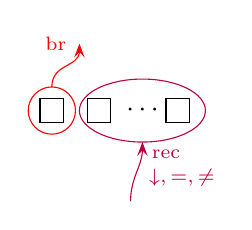
\begin{tikzpicture}
			\draw[red] (0.15,0.15) circle (0.3); 
			%		\node at (-0.2, -0.2) {\scriptsize\color{red} id};
			\node at (0.2, 1) {\scriptsize\color{red} br};
			\draw[purple] (1.3,0.15) ellipse (0.8 and 0.4);
			\node at (1.6, -0.4) {\scriptsize\color{purple} rec};
			\node at (1.8, -0.7) {\scriptsize\color{purple} $\downarrow, =, \neq$};
			
			\draw (0,0) rectangle (0.3,0.3);
			\draw (0.6,0) rectangle (0.9,0.3);
			\node at (1.3,0.15) {$\cdots$};
			\draw (1.6,0) rectangle (1.9,0.3);
			
			\draw[red, arrows = {-Stealth[length=5pt, inset=2pt]}] (0.15, 0.45) .. controls +(0,0.3) and +(0,-0.3) .. (0.5, 1); 
			\draw[purple, arrows = {-Stealth[length=5pt, inset=2pt]}] (1.15, -1) .. controls +(0,0.3) and +(0,-0.3) .. (1.3, -0.25); 
		\end{tikzpicture}
	\end{center}
	
	\pause
	\textbf{\small Messages received with the same value come from the same agent.}
\end{frame}



\subsection{Well quasi-orders}

\begin{frame}
	\tableofcontents[currentsubsection]
\end{frame}


\begin{frame}{Well quasi-orders}
		 
	
		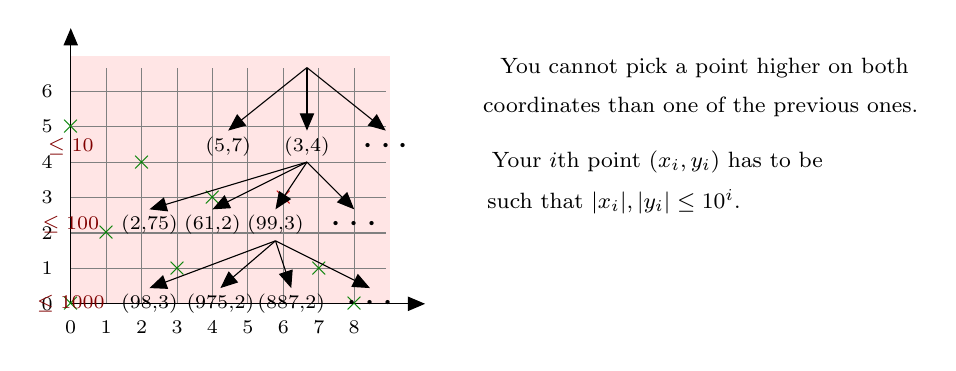
\begin{tikzpicture}[>= triangle 45]
	
\onslide<3-12>{\path [fill=red!10] (0.45*4, 0.45*3) rectangle (0.45*9, 0.45*7);}
\onslide<5-12>{\path [fill=red!10] (0.45*2, 0.45*4) rectangle (0.45*9, 0.45*7);}
\onslide<6-12>{\path [fill=red!10] (0.45*7, 0.45*1) rectangle (0.45*9, 0.45*7);}
\onslide<7-12>{\path [fill=red!10] (0.45*0, 0.45*5) rectangle (0.45*9, 0.45*7);}
\onslide<8-12>{\path [fill=red!10] (0.45*8, 0.45*0) rectangle (0.45*9, 0.45*7);}
\onslide<9-12>{\path [fill=red!10] (0.45*3, 0.45*1) rectangle (0.45*9, 0.45*7);}
\onslide<10-12>{\path [fill=red!10] (0.45*1, 0.45*2) rectangle (0.45*9, 0.45*7);}
\onslide<11-12>{\path [fill=red!10] (0.45*0, 0.45*0) rectangle (0.45*9, 0.45*7);}

\onslide<1-12>{
\draw[gray, step = 0.45] (0,0) grid (4,3);
\draw[->] (0,0) -- (4.5,0);
\draw[->] (0,0) -- (0,3.5);



\node (0) at (0*0.45,-0.3) {\scriptsize $0$};
\node (1) at (1*0.45,-0.3) {\scriptsize $1$};
\node (2) at (2*0.45,-0.3) {\scriptsize $2$};
\node (3) at (3*0.45,-0.3) {\scriptsize $3$};
\node (4) at (4*0.45,-0.3) {\scriptsize $4$};
\node (5) at (5*0.45,-0.3) {\scriptsize $5$};
\node (6) at (6*0.45,-0.3) {\scriptsize $6$};
\node (7) at (7*0.45,-0.3) {\scriptsize $7$};
\node (8) at (8*0.45,-0.3) {\scriptsize $8$};

\node (0) at (-0.3,0*0.45) {\scriptsize $0$};
\node (0) at (-0.3,1*0.45) {\scriptsize $1$};
\node (0) at (-0.3,2*0.45) {\scriptsize $2$};
\node (0) at (-0.3,3*0.45) {\scriptsize $3$};
\node (0) at (-0.3,4*0.45) {\scriptsize $4$};
\node (0) at (-0.3,5*0.45) {\scriptsize $5$};
\node (0) at (-0.3,6*0.45) {\scriptsize $6$};
}

\onslide<2-12> {\node[green!50!black] (0) at (0.45*4, 0.45*3) {$\times$};}
\onslide<4> {\node[red!80!black] (0) at (0.45*6, 0.45*3) {$\times$};}
\onslide<5-12> {\node[green!50!black] (0) at (0.45*2, 0.45*4) {$\times$};}
\onslide<6-12> {\node[green!50!black] (0) at (0.45*7, 0.45*1) {$\times$};}
\onslide<7-12> {\node[green!50!black] (0) at (0.45*0, 0.45*5) {$\times$};}
\onslide<8-12> {\node[green!50!black] (0) at (0.45*8, 0.45*0) {$\times$};}
\onslide<9-12> {\node[green!50!black] (0) at (0.45*3, 0.45*1) {$\times$};}
\onslide<10-12> {\node[green!50!black] (0) at (0.45*1, 0.45*2) {$\times$};}
\onslide<11-12> {\node[green!50!black] (0) at (0.45*0, 0.45*0) {$\times$};}

\onslide<3->{
\node (txt1) at (8, 3) {\footnotesize $\blacktriangleright$ You cannot pick a point higher on both} ;
\node (txt2) at (8, 2.5) {\footnotesize coordinates than one of the previous ones.} ;
}

\onslide<12->{
\node (txt1) at (7.4, 1.8) {\footnotesize $\blacktriangleright$ Your $i$th point $(x_i, y_i)$ has to be } ;
\node (txt2) at (6.9, 1.3) {\footnotesize such that $|x_i|, |y_i| \leq 10^i$.} ;
}

	\onslide<13->{
	\node (11) at (2,2) {\scriptsize(5,7)} ;
	\node (11) at (3,2) {\scriptsize(3,4)} ;
	\node (11) at (4,2) {\Large $\cdots$} ;
	
	\node (leq) at (0, 2) {\color{red!50!black}\scriptsize$\leq 10$};
	}

	\onslide<14->{
	\node (21) at (1,1) {\scriptsize(2,75)} ;
	\node (21) at (1.8,1) {\scriptsize(61,2)} ;
	\node (21) at (2.6,1) {\scriptsize(99,3)} ;
	\node (21) at (3.6,1) {\Large $\cdots$} ;
	\node (leq) at (0, 1) {\color{red!50!black}\scriptsize$\leq 100$};
	}

\onslide<15->{	
		\node (21) at (1,0) {\scriptsize(98,3)} ;
	\node (21) at (1.9,0) {\scriptsize(975,2)} ;
	\node (21) at (2.8,0) {\scriptsize(887,2)} ;
	\node (21) at (3.8,0) {\Large $\cdots$} ;
	\node (leq) at (0, 0) {\color{red!50!black}\scriptsize$\leq 1000$};
	}

\onslide<13-> {
	\draw[->] (3,3) -- (2,2.2);
	\draw[->] (3,3) -- (3,2.2);
	\draw[->] (3,3) -- (4,2.2);
}
\onslide<14-> {
	\draw[->] (3,1.8) -- (1,1.2);
	\draw[->] (3,1.8) -- (1.8,1.2);
	\draw[->] (3,1.8) -- (2.6,1.2);
	\draw[->] (3,1.8) -- (3.6,1.2);
}
\onslide<15->{
	\draw[->] (2.6,0.8) -- (1,0.2);
	\draw[->] (2.6,0.8) -- (1.9,0.2);
	\draw[->] (2.6,0.8) -- (2.8,0.2);
	\draw[->] (2.6,0.8) -- (3.8,0.2);
}

\end{tikzpicture}
		
		\onslide<1-12>{\onslide<2->{$(4,3)$}\onslide<4>{$\to {\color{red}(6,3)}$}\onslide<5->{\hspace{-1.35cm}$\to (2,4)$}\onslide<6->{$\to (7,1)$}\onslide<7->{$\to (0,5)$}\onslide<8->{$\to (8,0)$}\onslide<9->{$\to (3,1)$}\onslide<10->{$\to (1,2)$}\onslide<11->{$\to (0,0)$}}

\onslide<16->{König's lemma $\to$ this tree is finite. 

In fact, there is a computable bound on the length of the longest branch.
}


\onslide<17>{\textbf{We can enumerate all possible such trees!}}

%	
%\onslide<13>{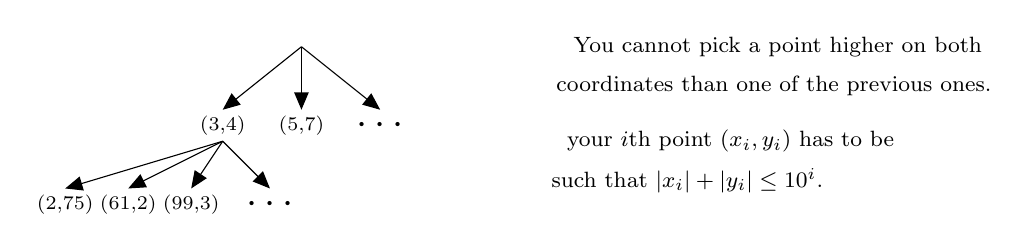
\begin{tikzpicture}[>= triangle 45]
	

\node (0) at (2,2.4) {};
\node (1) at (1,2) {\scriptsize(3,4)} ;
\node (1) at (2,2) {\scriptsize(5,7)} ;
\node (1) at (3,2) {\Large $\cdots$} ;

\node (2) at (-1,1) {\scriptsize(2,75)} ;
\node (2) at (-0.2,1) {\scriptsize(61,2)} ;
\node (2) at (0.6,1) {\scriptsize(99,3)} ;
\node (2) at (1.6,1) {\Large $\cdots$} ;


\draw[->] (2,3) -- (1,2.2);
\draw[->] (2,3) -- (2,2.2);
\draw[->] (2,3) -- (3,2.2);

\draw[->] (1,1.8) -- (-1,1.2);
\draw[->] (1,1.8) -- (-0.2,1.2);
\draw[->] (1,1.8) -- (0.6,1.2);
\draw[->] (1,1.8) -- (1.6,1.2);

	\node (txt1) at (8, 3) {\footnotesize $\blacktriangleright$ You cannot pick a point higher on both} ;
	\node (txt2) at (8, 2.5) {\footnotesize coordinates than one of the previous ones.} ;
	
	\node (txt1) at (7.4, 1.8) {\footnotesize $\blacktriangleright$ your $i$th point $(x_i, y_i)$ has to be } ;
	\node (txt2) at (6.9, 1.3) {\footnotesize such that $|x_i| + |y_i| \leq 10^i$.} ;
	
\end{tikzpicture}}
	
%	\vspace{1cm}\onslide<2->{$(4,3)$}\onslide<4>{$\to (4,2)$}\onslide<5->{\hspace{-1.35cm}$\to (2,4)$}\onslide<6->{$\to (7,1)$}\onslide<7->{$\to (0,5)$}\onslide<8->{$\to (8,0)$}\onslide<9->{$\to (3,1)$}\onslide<10->{$\to (1,2)$}\onslide<11->{$\to (0,0)$}
\end{frame}


\begin{frame}{Well quasi-orders: Subwords}
	
	\begin{block}{Higman's lemma}
		For all finite alphabet $\Sigma$, the subword order $\preceq$ is a well quasi-order over $\Sigma^*$.
	\end{block}

	\pause
	$\Leftrightarrow$ Any sequence $w_0, w_1, w_2, \ldots$ of words over $\Sigma$ such that $w_i \npreceq w_j$ for all $i<j$ is \textbf{finite}.
	
	\vspace{1cm}
	\pause
	Given a finite alphabet $\Sigma$ and a computable function $B : \mathbb{N} \to \mathbb{N}$, the set of sequences $(w_i)_{i \in \mathbb{N}}$ over $\Sigma$ such that
	\begin{itemize}
		\item $w_i \npreceq w_j$ for all $i<j$ 
		\item $|w_i| \leq B(i)$ for all $i$
	\end{itemize}
is finite and computable.
\end{frame}

\subsection{Decidability proof}

\begin{frame}
	\tableofcontents[currentsubsection]
\end{frame}

\begin{frame}{Towards a tree abstraction}
Assume that there is a valid run $\rho$ for COVER. 
\begin{block}{Observation 1}
If agent $a$ broadcasts to agents $b$ and $c$, we can make copy agent $a$ so that $b$ and $c$ receive messages from distinct agents. 
\end{block}
We can modify $\rho$ so that each agent sends messages to one single agent.
\pause

\begin{block}{Observation 2}
If $a$ broadcasts $m_1$ to $b$ then $b$ broadcasts $m_2$ to $a$, we can make a copy $a'$ of $a$ that broadcasts to $b$ and then stops; $a' \to b \to a$.
\end{block}
More generally, we can guarantee that the graph of ``who sends messages to whom'' has no cycle: it's a tree !
\end{frame}
	

\begin{frame}{Tree unfoldings}
	

	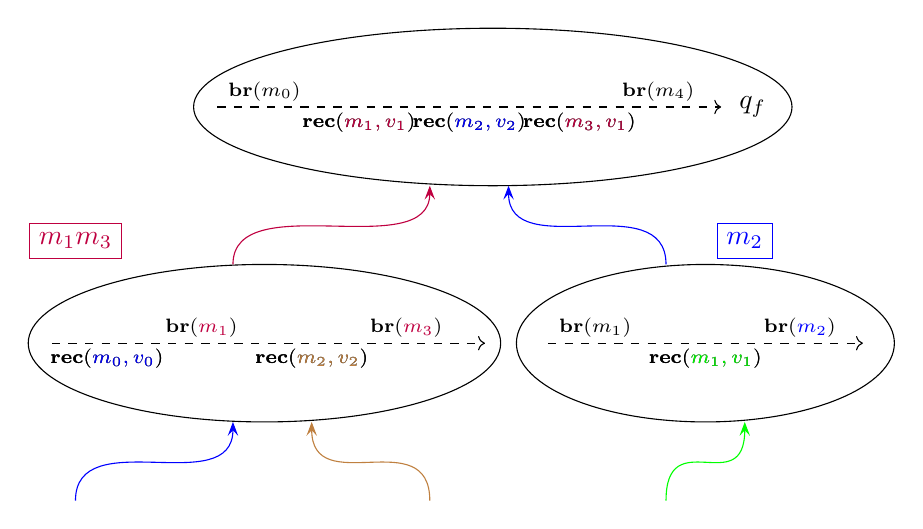
\begin{tikzpicture}
	
	\onslide<1-> 
	{
	\draw[->, dashed] (-0.2,0) -- (6.2,0);
	\node at (6.6,0) (qf) {$q_f$};
	\node (0) at (0.4,0.2) {\scriptsize $\br(m_0)$};
	\onslide<1>
	{
	\node (1) at (1.6,-0.2) {\scriptsize $\rec(m_1, v_1)$};
	\node (2) at (3,-0.2) {\scriptsize $\rec(m_2, v_2)$};
	\node (3) at (4.4,-0.2) {\scriptsize $\rec(m_3, v_1)$};
}
	\onslide<2->
	{
	\node (1) at (1.6,-0.2) {\scriptsize $\rec(\color{purple}m_1, v_1\color{black})$};
	\node (2) at (3,-0.2) {\scriptsize $\rec(\color{blue} m_2, v_2\color{black})$};
	\node (3) at (4.4,-0.2) {\scriptsize $\rec(\color{purple}m_3, v_1\color{black})$};
	}
	\node (4) at (5.4,0.2) {\scriptsize $\br(m_4)$};
	}
	
	
	
	\onslide<3-> 
	{
		\draw[->, dashed] (-2.3,-3) -- (3.2,-3);
		\node (0') at (-0.4,-2.8) {\scriptsize $\br(\color{purple}m_1\color{black})$};
		\node (1') at (-1.6,-3.2) {\scriptsize $\rec(m_0, v_0)$};
		\node (2') at (1,-3.2) {\scriptsize $\rec(m_2, v_2)$};
		\node (3') at (2.2,-2.8) {\scriptsize $\br(\color{purple}m_3\color{black})$};
	}
	
		\onslide<3-> 
	{
		\draw[->, dashed] (4,-3) -- (8,-3);
		\node (0'') at (4.6,-2.8) {\scriptsize $\br(\color{black}m_1\color{black})$};
		\node (2'') at (6,-3.2) {\scriptsize $\rec(m_1, v_1)$};
		\node (3'') at (7.2,-2.8) {\scriptsize $\br(\color{blue}m_2\color{black})$};
	}
	
	\onslide<4->
	{
		
		\draw (3.3,0) ellipse (3.8 and 1);
		\draw (0.4,-3) ellipse (3 and 1);
		\draw (6,-3) ellipse (2.4 and 1);
	\draw[purple, arrows = {-Stealth[length=5pt, inset=2pt]}] (0, -2) .. controls +(0,1) and +(0,-1) .. (2.5, -1); 
	\draw[blue, arrows = {-Stealth[length=5pt, inset=2pt]}] (5.5, -2) .. controls +(0,1) and +(0,-1) .. (3.5, -1);  
	
	\node[draw, purple] (Tp) at (-2,-1.7) {$m_1m_3$};
	\node[draw, blue] (Tb) at (6.5,-1.7) {$m_2$};
	% \node[draw, orange] (Tb) at (7,0) {$m$};
%	\draw[purple, arrows = {-Stealth[length=5pt, inset=2pt]}] (3.6, -1.7) .. controls +(0,1) and +(0,-1) .. (5.5, -0.4);
	}
	
	\onslide<5->
	{
		\draw[blue, arrows = {-Stealth[length=5pt, inset=2pt]}] (-2, -5) .. controls +(0,1) and +(0,-1) .. (0, -4); 
		\draw[brown, arrows = {-Stealth[length=5pt, inset=2pt]}] (2.5, -5) .. controls +(0,1) and +(0,-1) .. (1, -4);  
		\draw[green, arrows = {-Stealth[length=5pt, inset=2pt]}] (5.5, -5) .. controls +(0,1) and +(0,-1) .. (6.5, -4);  

		\node (1') at (-1.6,-3.2) {\scriptsize $\rec(\color{blue}m_0, v_0\color{black})$};
		\node (2') at (1,-3.2) {\scriptsize $\rec(\color{brown}m_2, v_2\color{black})$};
		\node (2'') at (6,-3.2) {\scriptsize $\rec(\color{green}m_1, v_1\color{black})$};
		
		%	\draw[purple, arrows = {-Stealth[length=5pt, inset=2pt]}] (3.6, -1.7) .. controls +(0,1) and +(0,-1) .. (5.5, -0.4);
	}
\end{tikzpicture}
	
\end{frame}

\begin{frame}{Tree unfoldings}
	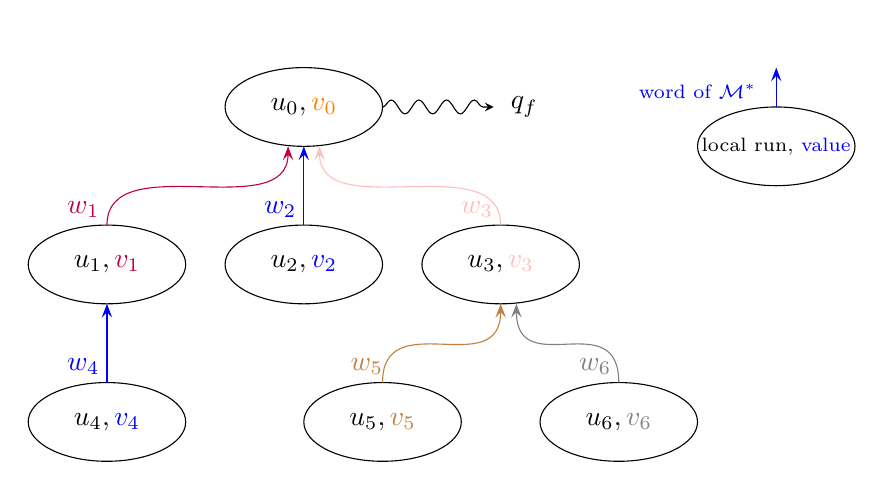
\begin{tikzpicture}
	
	\draw (1,0) ellipse (1 and 0.5);
	\node (u1) at (1,0) {$u_0,\color{orange} v_0$};
	
	\draw (-1.5,-2) ellipse (1 and 0.5);
	\node (u2) at (-1.5,-2) {$u_1, \color{purple} v_1$};
	
	\draw (1,-2) ellipse (1 and 0.5);
	\node (u3) at (1,-2) {$u_2, \color{blue} v_2$};
	
	\draw (3.5,-2) ellipse (1 and 0.5);
	\node (u4) at (3.5,-2) {$u_3, \color{pink} v_3$};
	
	\draw (2,-4) ellipse (1 and 0.5);
	\node (u6) at (2,-4) {$u_5, \color{brown}v_5$};
	
	\draw (-1.5,-4) ellipse (1 and 0.5);
	\node (u5) at (-1.5,-4) {$u_4, \color{blue}v_4$};
	
	\draw (5,-4) ellipse (1 and 0.5);
	\node (u7) at (5,-4) {$u_6, \color{gray}v_6$};
	
	
	\node (2) at (-1.8,-1.3) {\color{purple}$w_1$};
	\node (3) at (0.7,-1.3) {\color{blue}$w_2$};
	\node (4) at (3.2,-1.3) {\color{pink}$w_3$};
	\node (5) at (-1.8,-3.3) {\color{blue}$w_4$};
	\node (6) at (1.8,-3.3) {\color{brown}$w_5$};
	\node (7) at (4.7,-3.3) {\color{gray}$w_6$};
	\node (qf) at (3.8,0) {$q_f$};
	\draw[-stealth, decorate, decoration = snake] (2,0) -- (3.41,0);	
	

	\draw[blue, arrows = {-Stealth[length=5pt, inset=2pt]}] (-1.5, -3.5) .. controls +(0,1) and +(0,-1) .. (-1.5, -2.5); 
	
	
	\draw[brown, arrows = {-Stealth[length=5pt, inset=2pt]}] (2, -3.5) .. controls +(0,1) and +(0,-1) .. (3.5, -2.5);  
	\draw[gray, arrows = {-Stealth[length=5pt, inset=2pt]}] (5, -3.5) .. controls +(0,1) and +(0,-1) .. (3.7, -2.5); 
	
	\draw[blue, arrows = {-Stealth[length=5pt, inset=2pt]}] (1, -1.5) .. controls +(0,1) and +(0,-1) .. (1, -0.5); 
	\draw[purple, arrows = {-Stealth[length=5pt, inset=2pt]}] (-1.5, -1.5) .. controls +(0,1) and +(0,-1) .. (0.8, -0.5);  
	\draw[pink, arrows = {-Stealth[length=5pt, inset=2pt]}] (3.5, -1.5) .. controls +(0,1) and +(0,-1) .. (1.2, -0.5); 
	
	\begin{scope}[yshift = -1cm]
	\draw (7, 0.5) ellipse (1 and 0.5);
	\node (legend) at (7,0.5) {\scriptsize local run, \color{blue} value};
	\draw[blue, arrows = {-Stealth[length=5pt, inset=2pt]}] (7, 1) .. controls +(0,1) and +(0,-1) .. (7, 1.5); 
	\node (8) at (6, 1.2) {\color{blue}\scriptsize word of $\messages^*$};
	\end{scope}
\end{tikzpicture}
	
\end{frame}

\begin{frame}{Branch reduction}
	
	\begin{block}{Lemma}
		If a node labelled $w$ has a descendant labelled $w'$ with $w$ a subword of $w'$ then the tree can be reduced.
	\end{block}
	
	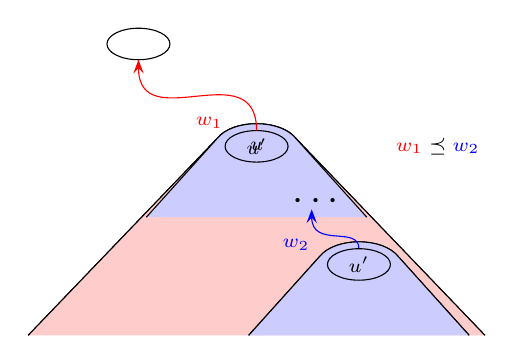
\begin{tikzpicture}
	
	\tikzset{every node/.style = {font = \scriptsize}}
	\onslide<2>
	{
		\draw (-0.4, -3.4) -- (2, -0.9) .. controls +(0.2,0.25) and +(-0.2,0.25) .. (3, -0.9) -- (5.4, -3.4); 
		\draw[fill=red!20] (-0.4, -3.4) -- (2, -0.9) .. controls +(0.2,0.25) and +(-0.2,0.25) .. (3, -0.9) -- (5.4, -3.4); 
		
		\draw (2.4, -3.4) -- (3.3, -2.4) .. controls +(0.2,0.25) and +(-0.2,0.25) .. (4.3, -2.4) -- (5.2, -3.4); 
		\draw[fill=blue!20] (2.4, -3.4) -- (3.3, -2.4) .. controls +(0.2,0.25) and +(-0.2,0.25) .. (4.3, -2.4) -- (5.2, -3.4); 
	}
	
	\onslide<3->
	{
%		\draw (-0.8, -3.8) -- (2, -0.9) .. controls +(0.2,0.25) and +(-0.2,0.25) .. (3, -0.9) -- (5.8, -3.8); 
		\draw[fill=blue!20] (1.1, -1.9) -- (2, -0.9) .. controls +(0.2,0.25) and +(-0.2,0.25) .. (3, -0.9) -- (3.9, -1.9); 
%		
%		\draw (2, -3.8) -- (3.3, -2.4) .. controls +(0.2,0.25) and +(-0.2,0.25) .. (4.3, -2.4) -- (5.6, -3.8); 
%		\draw[fill=blue!20] (2, -3.8) -- (3.3, -2.4) .. controls +(0.2,0.25) and +(-0.2,0.25) .. (4.3, -2.4) -- (5.6, -3.8); 
	}
	
	\draw (1,0.3) ellipse (0.4 and 0.2);
%	\node (u1) at (1,0) {$u_1,\color{orange} v_1$};
	
%	\draw (-1.5,-2) ellipse (1 and 0.5);
%	\node (u2) at (-1.5,-2) {$u_2, \color{purple} v_2$};
%	
%	\draw (1,-2) ellipse (1 and 0.5);
%	\node (u3) at (1,-2) {$u_3, \color{blue} v_3$};
%	
	\draw (2.5,-1) ellipse (0.4 and 0.2);
	\onslide<1-2>{\node (uv) at (2.5,-1) {\scriptsize $u$};}
	\onslide<3->{\node (uv) at (2.5,-1) {\scriptsize $u'$};}
%	\node (u4) at (3.5,-2) {$u_4, \color{pink} v_4$};
	
%	\node (u4) at (3.5,-2) {$u_4, \color{pink} v_4$};
%	
%	\draw (2,-4) ellipse (1 and 0.5);
%	\node (u6) at (2,-4) {$u_6, \color{brown}v_6$};
%	
%	\draw (-1.5,-4) ellipse (1 and 0.5);
%	\node (u5) at (-1.5,-4) {$u_5, \color{blue}v_5$};
%	
%	\draw (5,-4) ellipse (1 and 0.5);
%	\node (u7) at (5,-4) {$u_7, \color{gray}v_7$};
%	
	
%	\node (2) at (-1.8,-1.3) {\color{purple}$w_2$};
%	\node (3) at (0.7,-1.3) {\color{blue}$w_3$};
	\node (4) at (1.9,-0.7) {\color{red}$w_1$};
	\onslide<1-2>{\node (4) at (3,-2.25) {\color{blue}$w_2$};
		\draw[blue, arrows = {-Stealth[length=5pt, inset=2pt]}] (3.8, -2.3) .. controls +(0,0.3) and +(0,-0.5) .. (3.2, -1.8); 
		\node (dots) at (3.25, -1.7) {\Large$\cdots$};
		
		\draw (3.8,-2.5) ellipse (0.4 and 0.2);
		\node (u'v') at (3.8,-2.5) {\scriptsize $u'$};
	}
%	\node (5) at (-1.8,-3.3) {\color{blue}$w_5$};
%	\node (6) at (1.8,-3.3) {\color{brown}$w_6$};
%	\node (7) at (4.7,-3.3) {\color{gray}$w_7$};
%	\node (1) at (0.7,0.7) {\color{orange}$w_1$};	
	
	\node (txt) at (4.8,-1) {$\color{red} w_1 \color{black} \preceq \color{blue} w_2$};
%	
%	\draw[blue, arrows = {-Stealth[length=5pt, inset=2pt]}] (-1.5, -3.5) .. controls +(0,1) and +(0,-1) .. (-1.5, -2.5); 
%	
%	
%	\draw[brown, arrows = {-Stealth[length=5pt, inset=2pt]}] (2, -3.5) .. controls +(0,1) and +(0,-1) .. (3.5, -2.5);  
%	\draw[gray, arrows = {-Stealth[length=5pt, inset=2pt]}] (5, -3.5) .. controls +(0,1) and +(0,-1) .. (3.7, -2.5); 
%	
%	\draw[blue, arrows = {-Stealth[length=5pt, inset=2pt]}] (1, -1.5) .. controls +(0,1) and +(0,-1) .. (1, -0.5); 
%	\draw[purple, arrows = {-Stealth[length=5pt, inset=2pt]}] (-1.5, -1.5) .. controls +(0,1) and +(0,-1) .. (0.8, -0.5);  
	\draw[red, arrows = {-Stealth[length=5pt, inset=2pt]}] (2.5, -0.8) .. controls +(0,1) and +(0,-1) .. (1, 0.1); 
	

	
	
\end{tikzpicture}
\end{frame}

\begin{frame}{Branch reduction}
	\begin{itemize}
		\item We can assume that a node labelled $w$ has no descendant labelled $w' \succeq w$.
		\pause 
		\item In order to bound the size of the tree, we need a bound on the growth of the size of the nodes.
	\end{itemize}

	\pause

	\begin{block}{Shortening long local runs} There exists a primitive recursive function $\varphi: \mathbb{N} \rightarrow \mathbb{N}$ such that, if an agent must broadcast $k$ messages, its local run does not need to have more than $k \, \varphi(|\mathcal{P}|)$ steps. 
	\end{block}
	$|\mathcal{P}|$: size of the protocol \\
	Proof by shortening arguments (a bit involved)
\end{frame}

\begin{frame}{Bounding the branches}
	\centering
	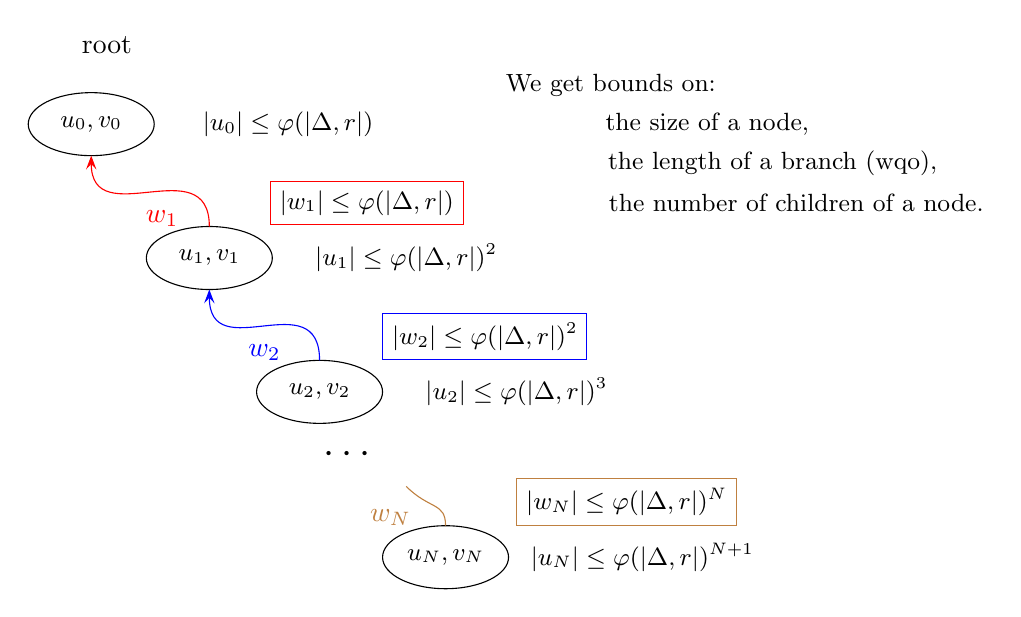
\begin{tikzpicture}
	
	\draw (1,0.5) ellipse (0.8 and 0.4);
	\draw (2.5,-1.2) ellipse (0.8 and 0.4);
	\draw (3.9,-2.9) ellipse (0.8 and 0.4);
	\draw (5.5,-5) ellipse (0.8 and 0.4);
	
	
	\node (uv) at (1,0.5) {\small $u_0,v_0$};
	\node (uv) at (2.5,-1.2) {\small $u_1,v_1$};
	\node (uv) at (3.9,-2.9) {\small $u_2,v_2$};
	\node (uv) at (5.5,-5) {\small $u_N,v_N$};
	
	
	\node (4) at (1.2,1.5) {root};
	
	\node (4) at (1.9,-0.7) {\color{red}$w_1$};
	\node (4) at (3.2,-2.4) {\color{blue}$w_2$};
	\node (4) at (4.8,-4.5) {\color{brown}$w_N$};
	
	\draw[blue, arrows = {-Stealth[length=5pt, inset=2pt]}] (3.9, -2.5) .. controls +(0,1) and +(0,-1) .. (2.5, -1.6); 
	\draw[red, arrows = {-Stealth[length=5pt, inset=2pt]}] (2.5, -0.8) .. controls +(0,1) and +(0,-1) .. (1, 0.1); 
	\draw[brown] (5.5, -4.6) .. controls +(0,0.3) and +(0.3,-0.3) .. (5, -4.1); 
	
	
	\onslide<2->
	{
		\node (uv) at (3.5,0.5) {\small $|u_0|\leq \varphi(|\Delta,r|)$};
	}
	\onslide<3->
	{
		\node[draw, color=red] (uv) at (4.5,-0.5) {\color{black}\small $|w_1|\leq \varphi(|\Delta,r|)$};
	}
	
	\onslide<4->
	{
		\node (uv) at (5,-1.2) {\small $|u_1| \leq \varphi(|\Delta,r|)^2$};
	}
	
	\onslide<5->
	{
		\node[draw, color=blue] (uv) at (6,-2.2) {\color{black}\small $|w_2|\leq \varphi(|\Delta,r|)^2$};
		\node[draw, color=brown] (uv) at (7.8,-4.3) {\color{black}\small $|w_N|\leq \varphi(|\Delta,r|)^{N}$};
		\node (uv) at (6.4,-2.9) {\small $|u_2| \leq \varphi(|\Delta,r|)^3$};
		\node (uv) at (8,-5) {\small $|u_N| \leq \varphi(|\Delta,r|)^{N+1}$};
	}
	
	\node (dots) at (4.25, -3.7) {\Large$\cdots$};
		
	\onslide<6->
	{
		\node (txt) at (7.6,1) {\small We get bounds on:};
		\node (txt) at (9.6,0) {\small $\blacktriangleright$ the length of a branch (wqo),};
		\node (txt) at (8.77,0.5) {\small $\blacktriangleright$ the size of a node,};
		\node (txt) at (9.9,-0.5) {\small $\blacktriangleright$ the number of children of a node.};
	}
	
	
	
\end{tikzpicture}

\end{frame}


\begin{frame}{Decidability}
	\begin{block}{Bounds}
	We use the previous argument to bound (in an irreducible tree):
	\begin{itemize}
	\item the length of all branches,
	\item the size of every node,
	\item the maximal degree of the tree.
	\end{itemize}
	This bounds the total space needed to store such a tree.
	\end{block}
	\pause 

	We can enumerate all irreducible trees in finite time, therefore
	
	\begin{block}{Theorem}
		The {\sc{Cover}} problem for \color{blue}signature \color{black} BNRA is decidable \onslide<3->{\color{red!70!black} and in $\mathbf{F}_{\omega^\omega}$.}
	\end{block} 
	\onslide<4->{Can be extended to the non-signature case.} 
\end{frame}

\section{Complexity bounds}



% \begin{frame}{Complexity bounds}
	
	
	
% 	\begin{block}{Length function theorem}
% 		For all finite $\Sigma$, for all $g : \mathbb{N} \to \mathbb{N}$ primitive recursive, there exists a function $F : \mathbb{N} \to \mathbb{N}$ of $\mathcal{F}_{\omega^{|\Sigma|-1}}$ such that for all $n \in \mathbb{N}$, every sequence $w_0, w_1, \ldots \in \Sigma^*$ such that $|w_i| \leq g^i(n)$ for all $i$ has at most $F(n)$ terms.\footnote{Cichon, Tahan Bittar, Theoretical Computer Science, '98}\footnote{Schmitz, Schnoebelen, ICALP'11}
% 	\end{block}
	
% 	\begin{itemize}
% 		\item We can bound the tree size by a function of $\mathcal{F}_{\omega^{\omega}}$.
% 	\end{itemize}
	
% %	\begin{block}{Lemma (Lower bound)}
% %		Reachability in Lossy channel systems is $\mathbf{F}_{\omega^\omega}$-complete.
% %	\end{block}
% %	
% %	\begin{itemize}
% %		\item We can encode LCS in BNRA by a PTIME reduction.
% %	\end{itemize}
% 	\pause
% 	\begin{block}{Theorem}
% 		{\sc{Cover}} in BNRA is $\mathbf{F}_{\omega^\omega}$-complete, even for a fixed number of registers $r\geq 2$.
% 	\end{block}
	
% 	\pause
	
% 	\begin{block}{Theorem}
% 		 {\sc{Cover}} in BNRA with one register is $\mathbf{NP}$-complete.
% 	\end{block}
% \end{frame}

\begin{frame}{Conclusion}
% \begin{itemize}
% 	\item Add mustard! \begin{itemize}
% 		\item Pushdown agents
% 		\item Inequality tests $\leq$
% 	\end{itemize} 
		
% 	\item Less permissive communication topology?
	
% 	\item Bounded number of alternations between broadcast and receive?
% \end{itemize} 

	\Huge \textbf{Thank you for your attention!}
\end{frame}

\appendix
 \begin{frame}
  
 \end{frame}
\begin{frame}{Complexity: encoding Lossy Channel Systems}
	Lossy Channel System = Transition system with FIFO memory + unreliable writes.\vspace{1cm}
	
	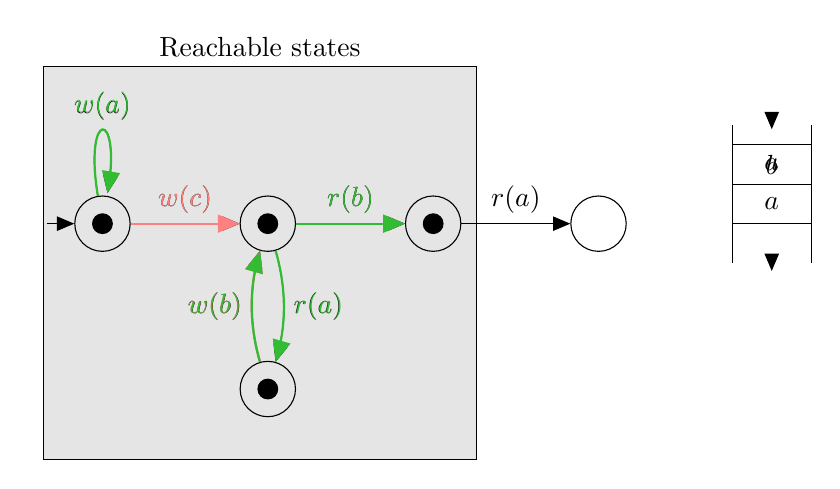
\begin{tikzpicture}[xscale=0.5,node distance=2.1cm,auto, AUT style,>= triangle
	45]
	\tikzstyle{initial}= [initial by arrow,initial text=,initial
	distance=.7cm]
	%	\tikzstyle{accepting}= [accepting by arrow,accepting text=,accepting
	%	distance=.7cm,accepting where =right]
	
	
	\onslide<10> {\draw[fill=gray!20] (-1.5, -3) rectangle (9.5, 2);
		\node (d) at (4,2.25) {Reachable states};
	}
	
	
	\node[state, initial, minimum width=0.1pt] (0) at (0,0) {};
	\node[state] [right of=0] (x) {};
	\node[state] [right of=x] (y) {};
	\node[state] [right of=y] (z) {};
	\node[state] [below of=x] (t) {};
	
	
	%	\path[->, bend left=10] 	
	%	(y) edge node[above] {$\mathbf{br}(b)$} (x)
	%	;
	
	\onslide<1,4-10>{\path[loop above] (0) edge node[above] {$w(a)$} (0);}
	\onslide<2-3>{\path[loop above,thick, color=RealGreen] (0) edge node[above] {\color{RealGreen}\textbf{$w(a)$}} (0);}
	
	\onslide<1-8,10>{\path[->] (x) edge node[above] {$r(b)$} (y);}
	\onslide<9>{\path[->, thick, color=RealGreen] (x) edge node[above] {\color{RealGreen}\textbf{$r(b)$}} (y);}
	
	\onslide<1-3,5-10>{\path[->] (0) edge node[above] {$w(c)$} (x);}
	\onslide<4>{\path[->, thick, color=red!50] (0) edge node[above] {\color{red!50}\textbf{$w(c)$}} (x);}
	
	\path[->] (y) edge node[above] {$r(a)$} (z);
	
	
	\onslide<1-4,6,8-10>{\path[->, bend left] (x) edge node[right] {$r(a)$} (t);}
	\onslide<5,7>{\path[->, bend left,thick, color=RealGreen] (x) edge node[right] {\color{RealGreen}\textbf{$r(a)$}} (t);}
	
	\onslide<1-5,7,9-10>{\path[->, bend left] (t) edge node[left] {$w(b)$} (x);}
	\onslide<6>{\path[->, bend left,thick, color=red!50] (t) edge node[left] {\color{red!50}\textbf{$w(b)$}} (x);}
	\onslide<8>{\path[->, bend left,thick, color=RealGreen] (t) edge node[left] {\color{RealGreen}\textbf{$w(b)$}} (x);}
	
	
	
	\onslide<3-4>
	{
	\draw (16,0) rectangle (18,0.5);
	\node at (17,0.25) {$a$};
}
	\onslide<2-6,8>
	{
	\draw (16,0.5) rectangle (18,1);
}
\onslide<2-6>
{
	\node at (17, 0.75) {$a$};
}
\onslide<8>
{
	\node at (17, 0.75) {$b$};
}


\onslide<1-3>
{
	\draw[fill=black] (0,0) ellipse (0.25 and 0.125);
}

\onslide<4,6,8>
{
	\draw[fill=black] (4.2,0) ellipse (0.25 and 0.125);
}

\onslide<5,7>
{
	\draw[fill=black] (4.2,-2.1) ellipse (0.25 and 0.125);
}

\onslide<9>
{
	\draw[fill=black] (8.4,0) ellipse (0.25 and 0.125);
}

\draw (16,-0.5) -- (16, 1.25);
\draw (18,-0.5) -- (18, 1.25);

\draw[->] (17, -0.4) -- (17, -0.6);
\draw[->] (17, 1.4) -- (17, 1.2);


\end{tikzpicture}
\end{frame}


\begin{frame}{Complexity: encoding Lossy Channel Systems}
	We simulate an LCS through a chain of agents that each apply a transition.
	
	Each agent stores:
	\begin{itemize}
		\item An identifier for itself
		
		\item Its predecessor's identifier
	\end{itemize} 
	
	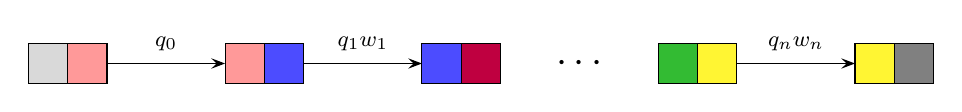
\begin{tikzpicture}

\draw[white, fill=gray!30] (0,0) rectangle (0.5,0.5);
\draw[white, fill=red!40] (2.5,0) rectangle (3,0.5);
\draw[white, fill=blue!70] (5,0) rectangle (5.5,0.5);
\draw[white, fill=RealGreen] (8,0) rectangle (8.5,0.5);
\draw[white, fill=yellow!80] (10.5,0) rectangle (11,0.5);

\draw[white, fill=red!40] (0.5,0) rectangle (1,0.5);
	\draw[white, fill=blue!70] (3,0) rectangle (3.5,0.5);
\draw[white, fill=purple] (5.5,0) rectangle (6,0.5);
\draw[white, fill=yellow!80] (8.5,0) rectangle (9,0.5);
\draw[white, fill=gray] (11,0) rectangle (11.5,0.5);
	
\draw (0,0) rectangle (1,0.5);
\draw (2.5,0) rectangle (3.5,0.5);
\draw (5,0) rectangle (6,0.5);
\draw (8,0) rectangle (9,0.5);
\draw (10.5,0) rectangle (11.5,0.5);

\draw (0.5,0) -- (0.5,0.5);
\draw (3,0) -- (3,0.5);
\draw (5.5,0) -- (5.5,0.5);
\draw (8.5,0) -- (8.5,0.5);
\draw (11,0) -- (11,0.5);


\draw[->, arrows = {-Stealth[length=5pt, inset=2pt]}] (1,0.25) -- (2.5,0.25);
\draw[->, arrows = {-Stealth[length=5pt, inset=2pt]}] (3.5,0.25) -- (5,0.25);
\draw[->, arrows = {-Stealth[length=5pt, inset=2pt]}] (9,0.25) -- (10.5,0.25);
	
\node (D) at (7,0.25) {\Large$\cdots$};

\node (X) at (1.75,0.5) {\footnotesize $q_0$};
\node (Y) at (4.25,0.5) {\footnotesize $q_1 w_1$};
\node (Z) at (9.75,0.5) {\footnotesize $q_{n} w_{n}$};
\end{tikzpicture}
	
\end{frame}

\begin{frame}{Complexity: encoding Lossy Channel Systems}
	
	\begin{tikzpicture}[xscale=0.5,node distance=2.1cm,auto, AUT style,>= triangle
	45]
	\tikzstyle{initial}= [initial by arrow,initial text=,initial
	distance=.7cm]
	%	\tikzstyle{accepting}= [accepting by arrow,accepting text=,accepting
	%	distance=.7cm,accepting where =right]
	
	
	\node[state, initial, minimum width=0.1pt] (0) at (0,0) {};
	\node[state] [right of=0] (l1) {};
	\node[state] [below of=0] (t1) {};
	\node[state] [right of=t1] (t2) {};
	\node[state] [right of=t2] (t3) {};
	\node[state] [right of=t3] (t4) {};
	
	

	\path[->] (0) edge node[above] {$\mathbf{br}(q_0, \reg_2)$} (l1);
	
	\path[->] (0) edge node[left] {$\mathbf{rec}(q, \downarrow\reg_1)$} (t1);
	\path[->] (t1) edge node[above] {$\mathbf{br}(q', \reg_2)$} (t2);
	\path[->] (t2) edge node[above] {$\mathbf{br}(a, \reg_2)$} (t3);
	\path[->, bend right=20] (t3) edge node[below] {$\mathbf{rec}(x, =\reg_1)$} (t4);
	\path[->, bend right=20] (t4) edge node[above] {$\mathbf{br}(x, \reg_2)$} (t3);
	
	\onslide<2>{
	\draw (-5,-3.5) rectangle (14, -0.5);
	\node (d) at (3,-4) {For each transition $q \xrightarrow{w(a)} q'$ of the LCS};
}
\end{tikzpicture}
	
\end{frame}

\begin{frame}{Complexity results}
	
	$\mathbf{F}_{\omega^\omega}$ = Hyper-Ackermannian complexity class.
	
	\begin{block}{Theorem}
		LCS reachability is $\mathbf{F}_{\omega^\omega}$-hard\footnote{Schnoebelen, Information agenting Letters '08}.
	\end{block}
	\pause 

	\begin{block}{Theorem}
		{\sc{Cover}} in BNRA is $\mathbf{F}_{\omega^\omega}$-complete, even for signature protocols with two registers.
	\end{block}
	\pause 

	\begin{block}{Theorem}
		 {\sc{Cover}} in BNRA with one register is $\mathbf{NP}$-complete.
	\end{block}
	
\end{frame}

\end{document}